\section{Gestione nodo}
Per quanto riguarda la gestione dei nodi l'utente ha la possibilità di:
\begin{itemize}
	\item aggiungere un \mglo{Nodo}{nodo};
	\item visualizzare i dettagli relativi a un certo nodo presente;
	\item modificare un nodo presente;
	\item eliminare un nodo presente.
\end{itemize}

\subsection{Aggiunta di un nodo}
Per aggiungere un nodo si deve:
\begin{itemize}
	\item cliccare sul pulsante "+" in basso a destra della mappa;
	\item selezionare la voce "Aggiungi nodo";
	\item posizionare il nodo sulla mappa all'interno di un \mglo{Asset}{asset};
	\item compilare i campi (tutti) rispettando i vincoli esposti nell'apposita appendice \nameref{Validazioni};
	\item cliccare sul pulsante "Salva", che verrà abilitato solo nel momento in cui tutte le operazioni sopra descritte sono state eseguite in maniera corretta.
\end{itemize}

\begin{figure}[H]
\centering
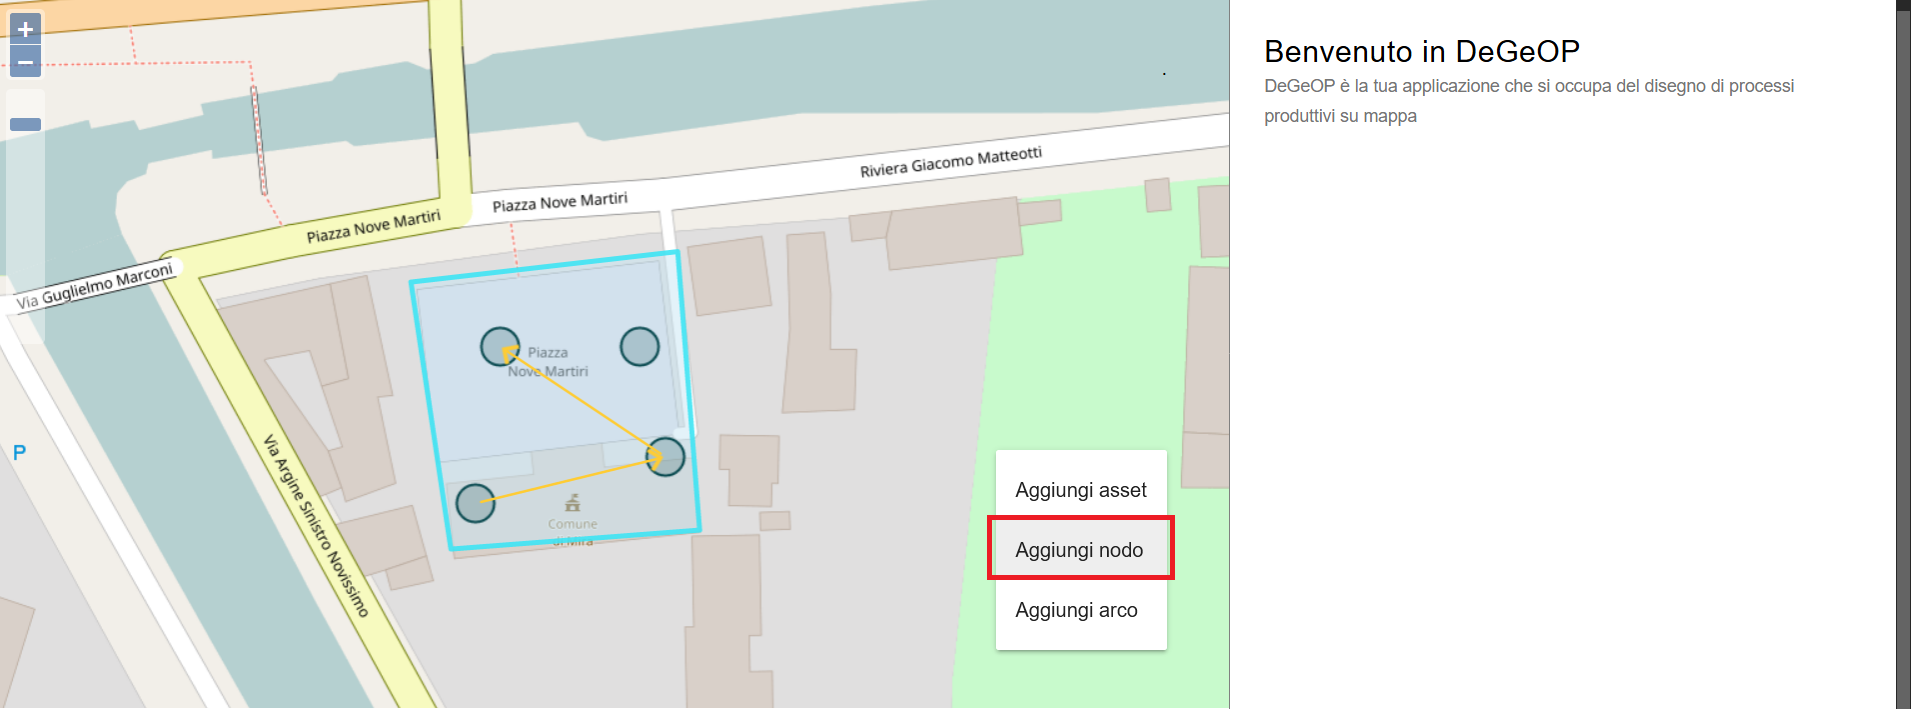
\includegraphics[width=\textwidth]{img/menu_aperto_nodo_hover.png}
\caption{Menu di aggiunta}
\end{figure}

\begin{figure}[H]
\centering
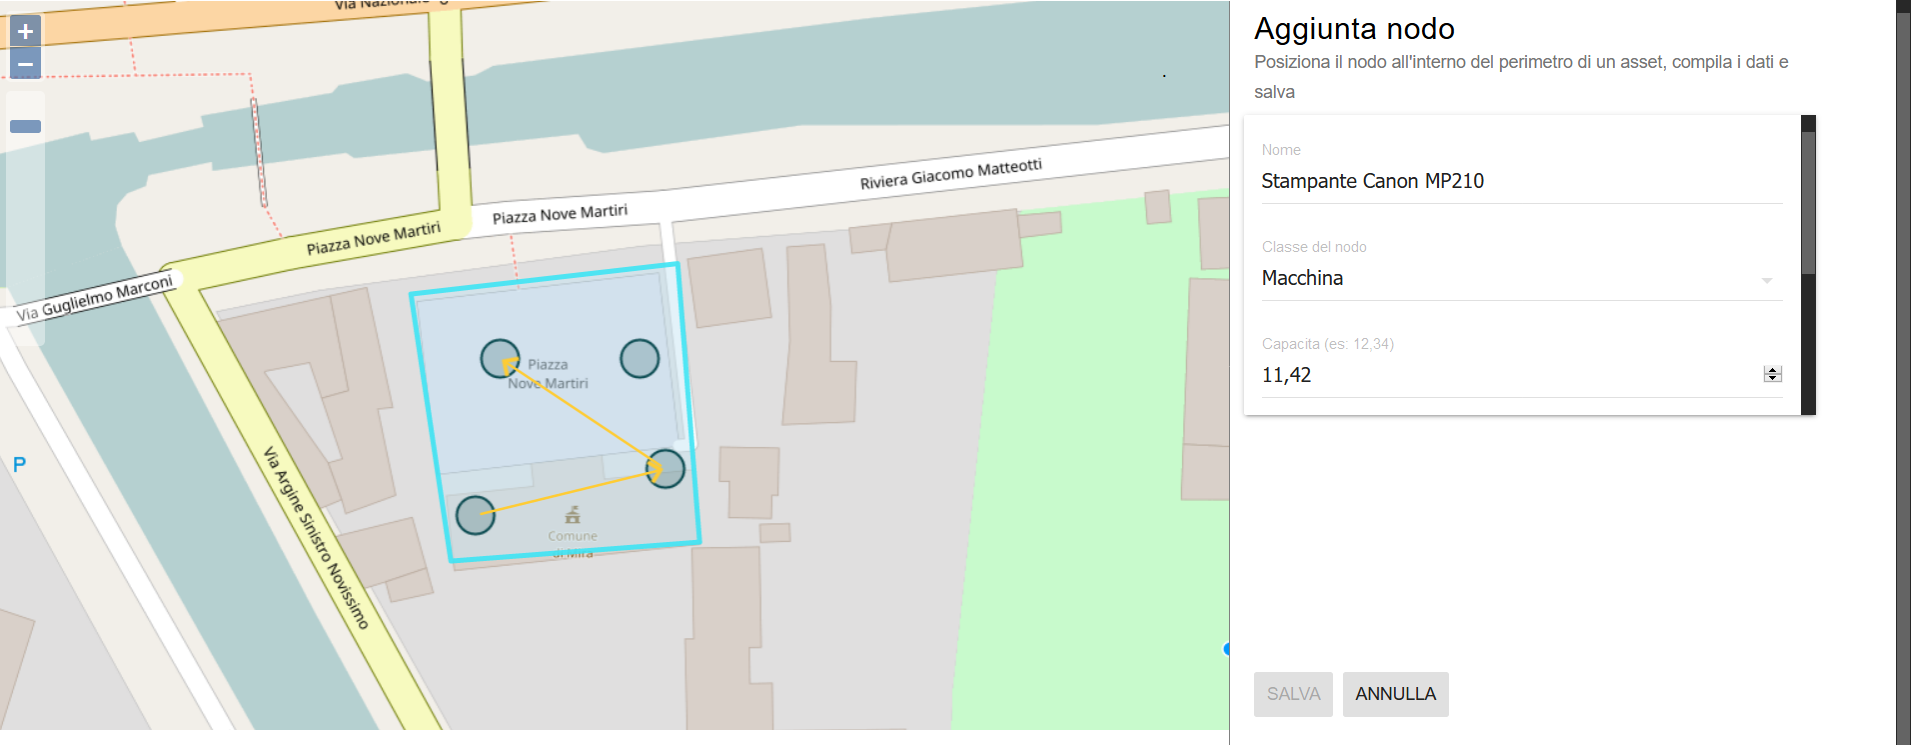
\includegraphics[width=\textwidth]{img/aggiunta_nodo.png}
\caption{Aggiunta di un nodo}
\end{figure}

\subsection{Visualizzazione dei dettagli di un nodo}
Per visualizzare i dettagli di un nodo si deve:
\begin{itemize}
	\item selezionare il  nodo che si intende modificare cliccando direttamente su quel nodo dalla mappa.
\end{itemize}

\begin{figure}[H]
\centering
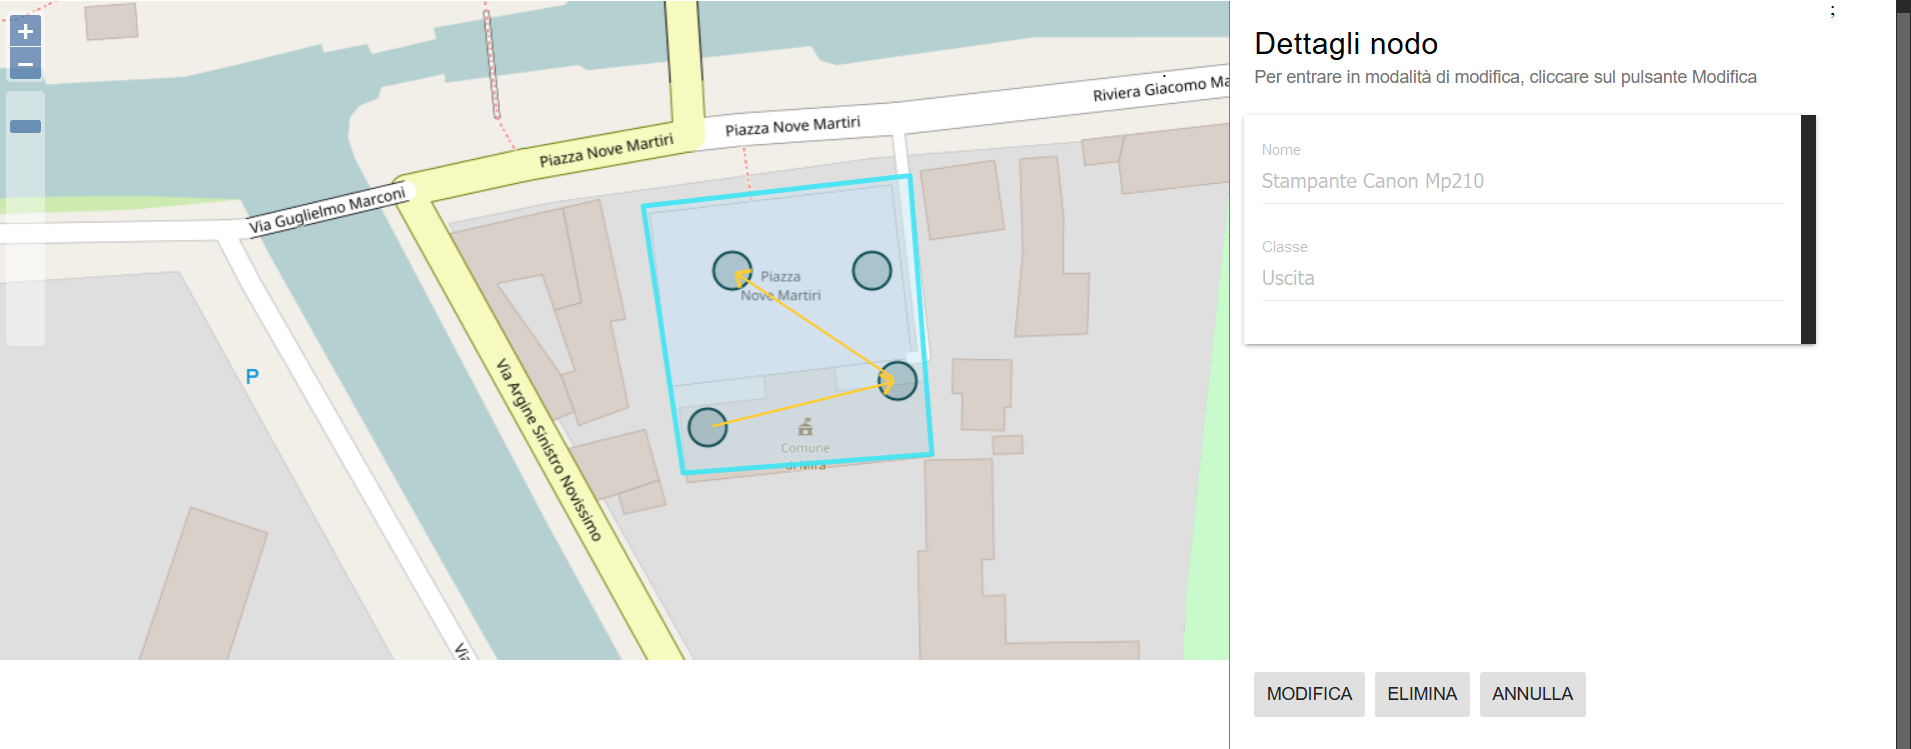
\includegraphics[width=\textwidth]{img/visualizzazione_nodo.png}
\caption{Visualizzazione dettagli di un nodo}
\end{figure}

\subsection{Modifica di un nodo}
Per modificare un nodo si deve:
\begin{itemize}
	\item selezionare il nodo che si intende modificare cliccando direttamente sulla mappa;
	\item cliccare sul pulsante "Modifica" in basso sulla sidebar;
	\item eventualmente riposizionare il perimetro del nodo sulla mappa all'interno di un certo asset. La nuova posizione andrà in automatico a sovrascrivere quello precedentemente presente.
	\item eventualmente modificare i campi rispettando i vincoli esposti nell'apposita appendice \nameref{Validazioni};
	\item cliccare sul pulsante "Salva", che verrà abilitato solo nel momento in cui tutte le operazioni sopra descritte sono state eseguite in maniera corretta.
\end{itemize}

\begin{figure}[H]
\centering
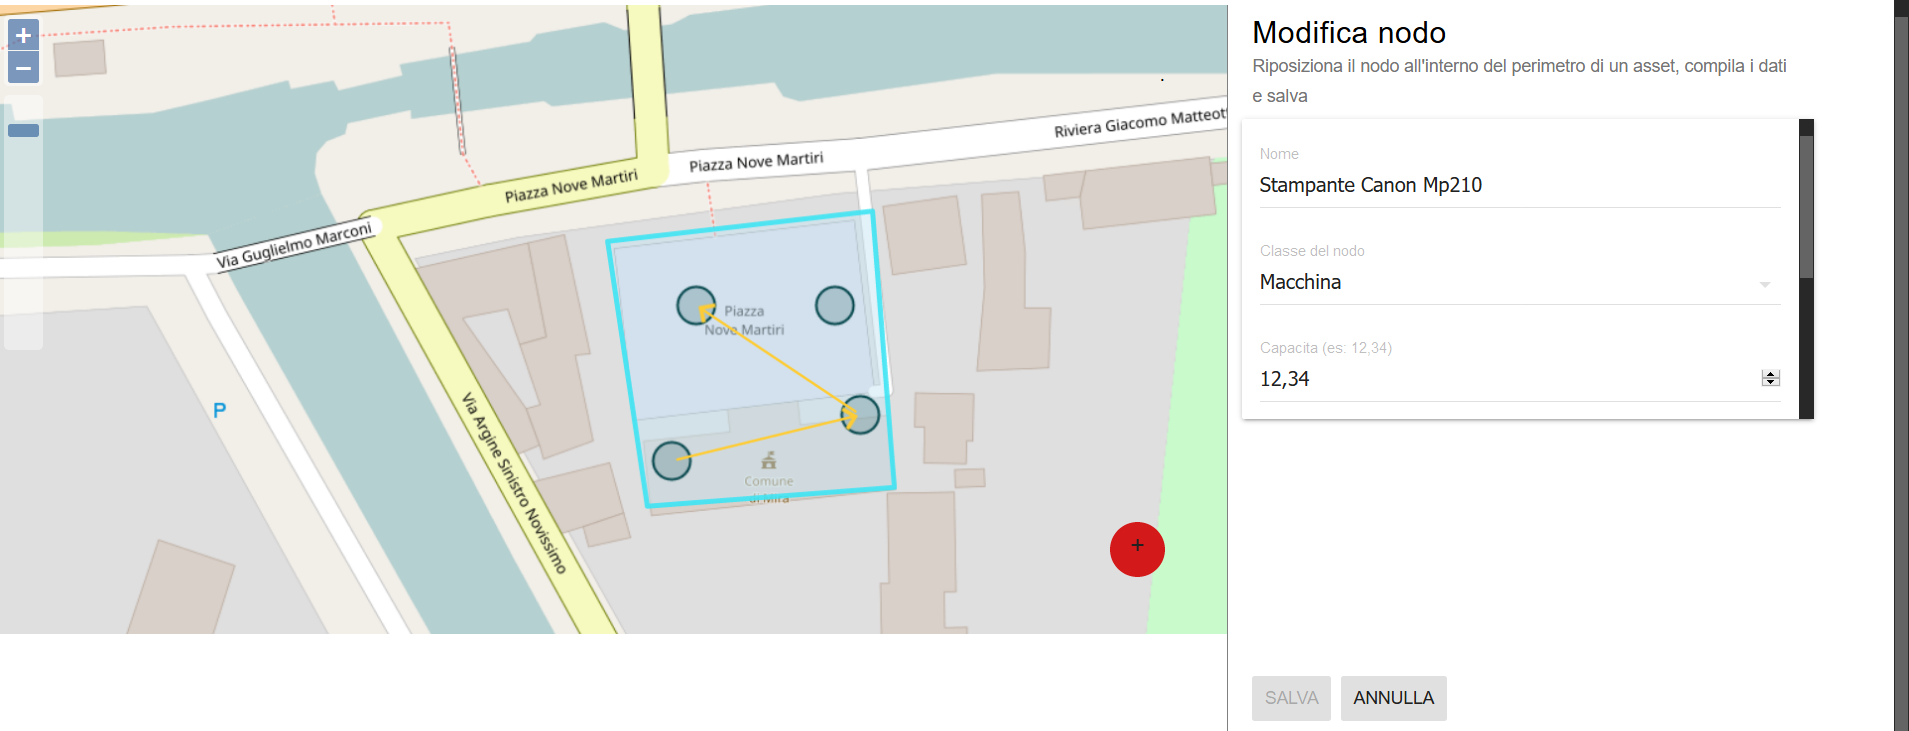
\includegraphics[width=\textwidth]{img/modifica_nodo.png}
\caption{Modifica di un nodo}
\end{figure}

\subsection{Eliminazione di un nodo}
Per eliminare un nodo si deve:
\begin{itemize}
	\item selezionare  nodo che si intende modificare cliccando direttamente sulla mappa;
	\item cliccare sul pulsante "Elimina" in basso sulla sidebar;
	\item cliccare sul pulsante "Elimina" sulla finestra bloccante che compare.
\end{itemize}

\begin{figure}[H]
\centering
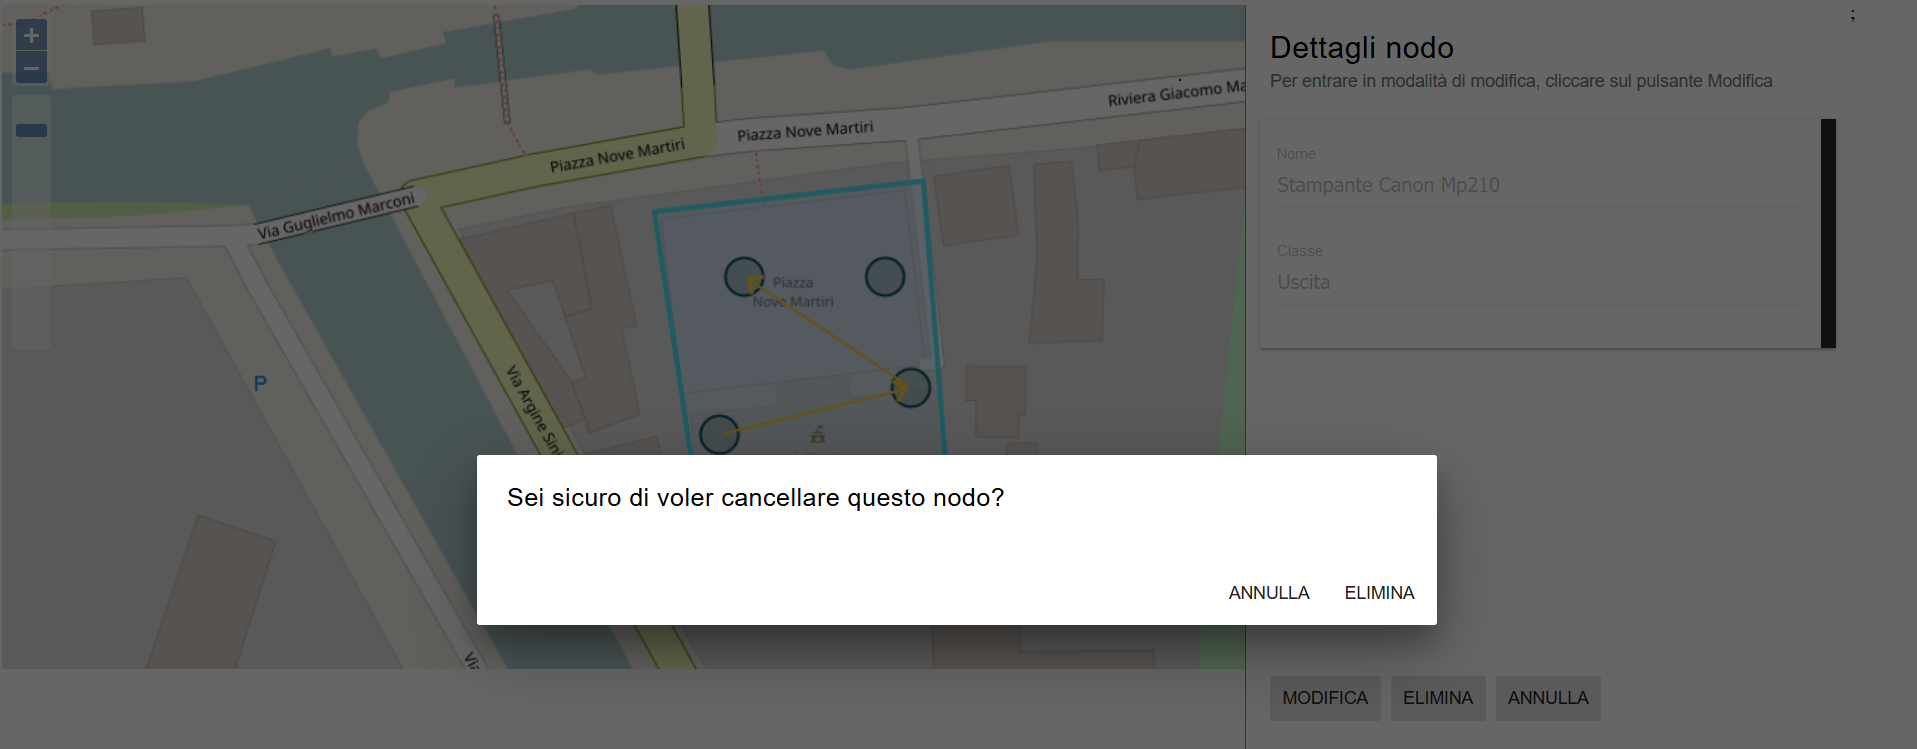
\includegraphics[width=\textwidth]{img/eliminazione_bloccante_nodo.png}
\caption{Eliminazione di un nodo}
\end{figure}